\chapter{Introduzione}
\epigraph{All men are really most attracted by the beauty of plain speech.}{Thoreau}

\section{Natural Language Processing}

L'elaborazione del linguaggio naturale (da qui in avanti \emph{NLP}, Natural Language Processing) è la parte delle scienze informatiche che si occupa dell'interazione tra macchina e linguaggio umano. Da questa premessa segue immediatamente che NLP è correlata all'ambito dell'interazione uomo-macchina.

Con ``linguaggio umano'' intendiamo una lingua che viene usata per le comunicazioni di tutti i giorni dagli umani, per esempio l'italiano, l'inglese o l'hindi. A differenza dei linguaggi artificiali, come i linguaggi di programmazione o le notazioni matematiche, i linguaggi naturali sono difficilmente fissabili in un insieme finito di regole. Questi ultimi infatti hanno un'infinità di varianti e, per di più, evolvono con il passare del tempo.

NLP può variare dall'essere estremamente facile all'estremamente difficile: da un lato potremmo confrontare due diversi stili di scrittura semplicemente contando le frequenze delle parole, dall'altro potremmo voler essere in grado di dare risposte sensate a qualsiasi quesito pronunciato da un umano.

Per capire quanti problemi ci sono all'interno dell'NLP proviamo a elencarne alcuni tra i più comuni:
\begin{itemize}
	\item Traduzione automatica: siamo abituati a poter tradurre automaticamente del testo da un linguaggio umano all'altro, ad esempio con Google Translate.
	\item Generazione di linguaggio naturale: gli assistenti vocali recuperano informazioni da svariate basi di dati e le presentano sotto forma di testo in un linguaggio umano.
	\item OCR (riconoscimento ottico dei caratteri): data un'immagine contenente del testo, stampato o scritto, ricavare il testo corrispondente.
	\item POS (Part Of Speech): data una frase, determinare la parte del discorso di ciascuna parola (verbo, nome, \dots) in modo analogo a quanto si fa nell'analisi grammaticale. 
	\item Divisione in frasi, riconoscendo gli opportuni segni di interpunzione.
	\item Riconoscimento vocale: partendo da una sorgente audio si vuole ottenere una trascrizione fedele a quanto pronunciato. Questo compito richiede a sua volta che sia risolto il problema di individuare, all'interno di un frammento audio, la corretta divisione delle parole.
	\item Classificazione del testo: se arriva una mail il cui oggetto contiene parole come ``Diventa subito milionario'' oppure ``Hai ereditato in Nigeria una somma di denaro'', il messaggio dovrebbe essere automaticamente riconosciuto come spam.
	\item Sentiment analysis: identificare la posizione soggettiva (cosiddetta polarizzazione) partendo da un testo. Un esempio può essere l'individuare lo stato emotivo di una persona (triste, arrabbiato, felice, ansioso, \dots) partendo da un tweet.	
	
\end{itemize} 

\section{Il problema della correzione automatica}

Ogni elaboratore di testi moderno che si rispetti include oggigiorno un potente correttore ortografico. Simili strumenti sono integrati anche nei browser e soprattutto nelle tastiere intelligenti degli smartphone. Nonostante sembrino utili, tutti odiano i correttori ortografici perché sono ritenuti ``stupidi''.

Il grosso equivoco di fondo è che il pubblico generalista non conosce i retroscena della correzione automatica e tende quindi a considerarlo un compito come gli altri, avente un esito binario: funziona oppure non funziona. Spesso si sottovaluta che i correttori ortografici automatici sono uno degli ambiti dell'intelligenza artificiale (AI) e nei lavori di AI, allo stato dell'arte, non è possibile ottenere una precisione del 100\%. Si punta, per quanto possibile, a rendere questa percentuale più alta possibile per fornire un risultato di qualità.

Kukich, nel suo articolo pubblicato nel 1992 \cite{kukich}, divide il problema generale della correzione in tre sottoproblemi via via più ampi e difficili:
\begin{itemize}
	\item Rilevamento dei ``non-word error'': rilevare errori che diventano parole sconosciute (come \emph{esmpio} al posto di \emph{esempio}).
	\item Correzione dei ``non-word error'': correggere le parole che diventano parole sconosciute osservando l'errore di per sè (correggere \emph{esmpio} in \emph{esempio}).
	\item Rilevamento e correzione basata sul contesto: usare il contesto per decidere se rilevare e correggere una parola anche qualora questa sia stata sfortunatamente trasformata in un'altra parola esistente (``real-word error''). Consideriamo come esempio il caso in cui \emph{tre} è stato scritto senza la prima lettera (\emph{re}).
\end{itemize}

\begin{figure}[!h]
\centering
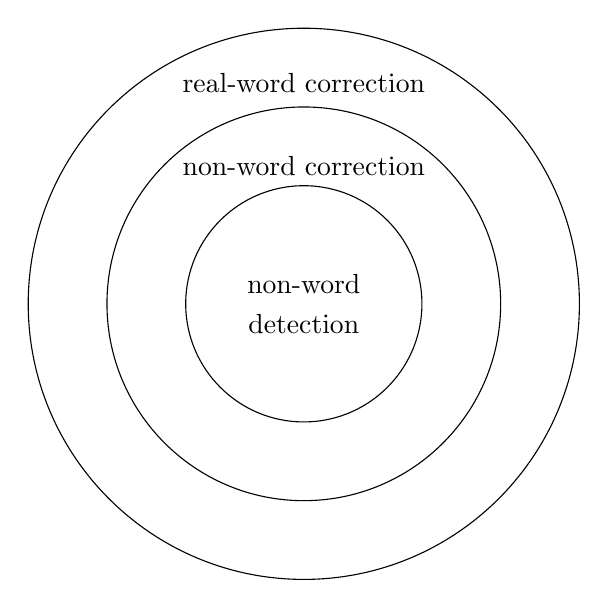
\begin{tikzpicture}
\foreach \r in {1.5,2.5,3.5}{
\draw (0,0) circle (\r cm);
}
\draw node[yshift=0.25cm]{non-word};
\draw node[yshift=-0.25cm]{detection};
\draw node[yshift=1.75cm]{non-word correction};
\draw node[yshift=2.80cm]{real-word correction};
\end{tikzpicture}
\caption{Diversi tipi di correzione automatica}
\end{figure}


Obiettivo di questo lavoro è arrivare a un sistema che provi a rispondere a tutte le richieste sopra descritte.